\clearpage
\section{Context of use}
\subsection{Idea of the application}
The idea behind Rent and Lend describes a software with the help of which one can lend tools to neighbors and borrow tools from neighbors.\\
Products on offer in the vicinity are to be displayed. The exchange with the other person is to take place via a chat. 
\subsection{User roles}
There are two user roles that can use the application. On the one hand there is the person who offers products to borrow. And on the other side there are people who can borrow these products.\\
It is important to say that these two roles can also overlap. 
\subsubsection{Lender}
Lenders offer products. They provide the things that can be lent. \\
A lending person has the concern that their products are easily found and they are contacted by many interested people. It is also important to ensure that their tools are handled with care. A lender wants to be confident that they will get their money and that their items will not be stolen or damaged. For these reasons, the lender may need more frequent service and support.
\subsubsection{Renter}
The borrowing person has the concern to find items quickly and easily. He wants the details of a product to be easy to read and at a glance.\\
 Furthermore, he hopes to be able to reach the lender fast and reliable. The goods should be as described and he should not be held responsible for any damage that the equipment has had before.

\subsection{User journey maps}
		For a greater understanding of future design choices and possible requirements, a user journey map for the lending and renting part of the application is created respectively. The different phases a user traverses are defined in the first step. The second step consists of finding possibles activities the user performs in the phases. In the last step the users feelings while performing the activities are depicted. This helps finding possible phases of the journey that may be difficult and finding a solution to simplify these phases.\\
		
		\subsubsection{User journey map for the renting person}
			This journey map consists of the following phases with the related activities:
			
			\begin{figure}[H]
				\centering
				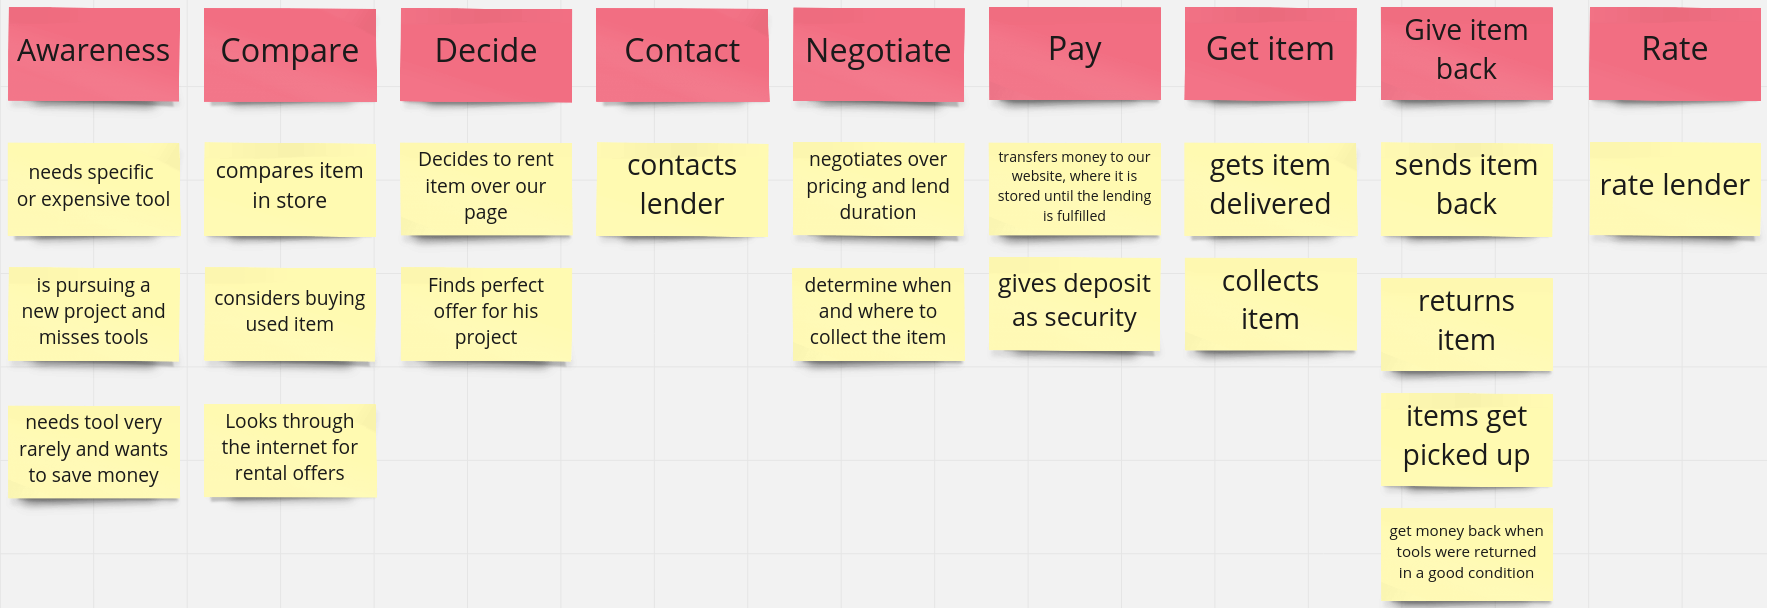
\includegraphics[width=\linewidth]{abb/2_context_of_use/user_journey_map_renting.png}
				\caption{User journey map for renting user}
				\label{fig:ujm_renting}
			\end{figure}
			
			\noindent
			The corresponding feelings and the graph are determined this way:
			
			\begin{figure}[H]
				\centering
				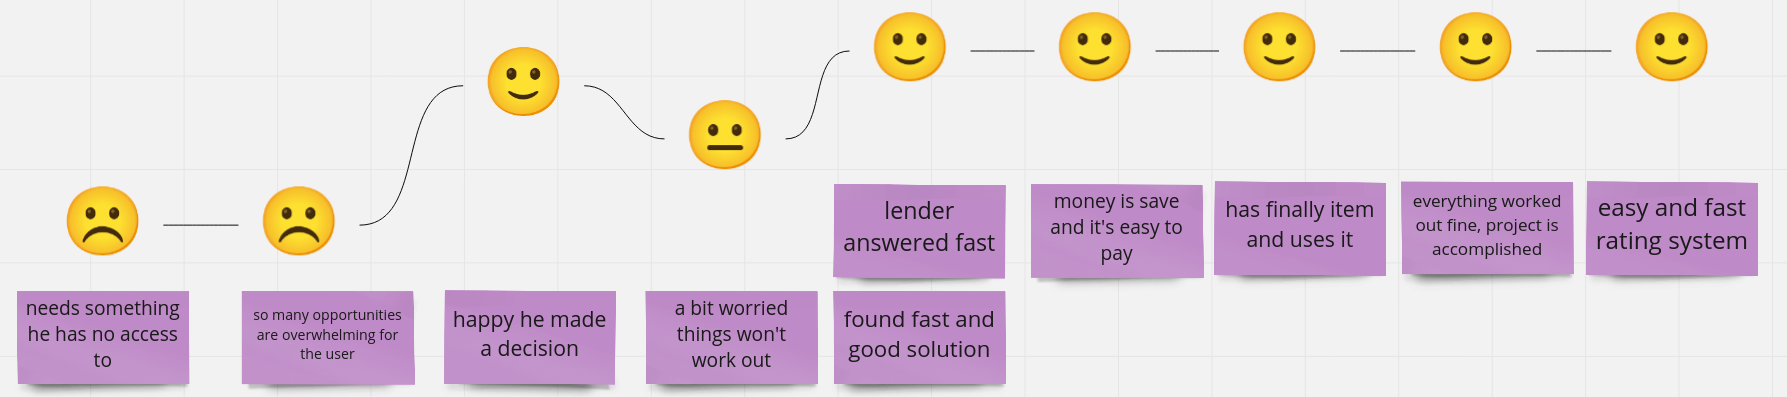
\includegraphics[width=\linewidth]{abb/2_context_of_use/feelings_renting.png}
				\caption{Feelings for renting user}
				\label{fig:ujm_renting_feelings}
			\end{figure}
		
		\subsubsection{User journey map for the renting person}
			The counterparts for the renting persons journey looks like this:
			
			\begin{figure}[H]
				\centering
				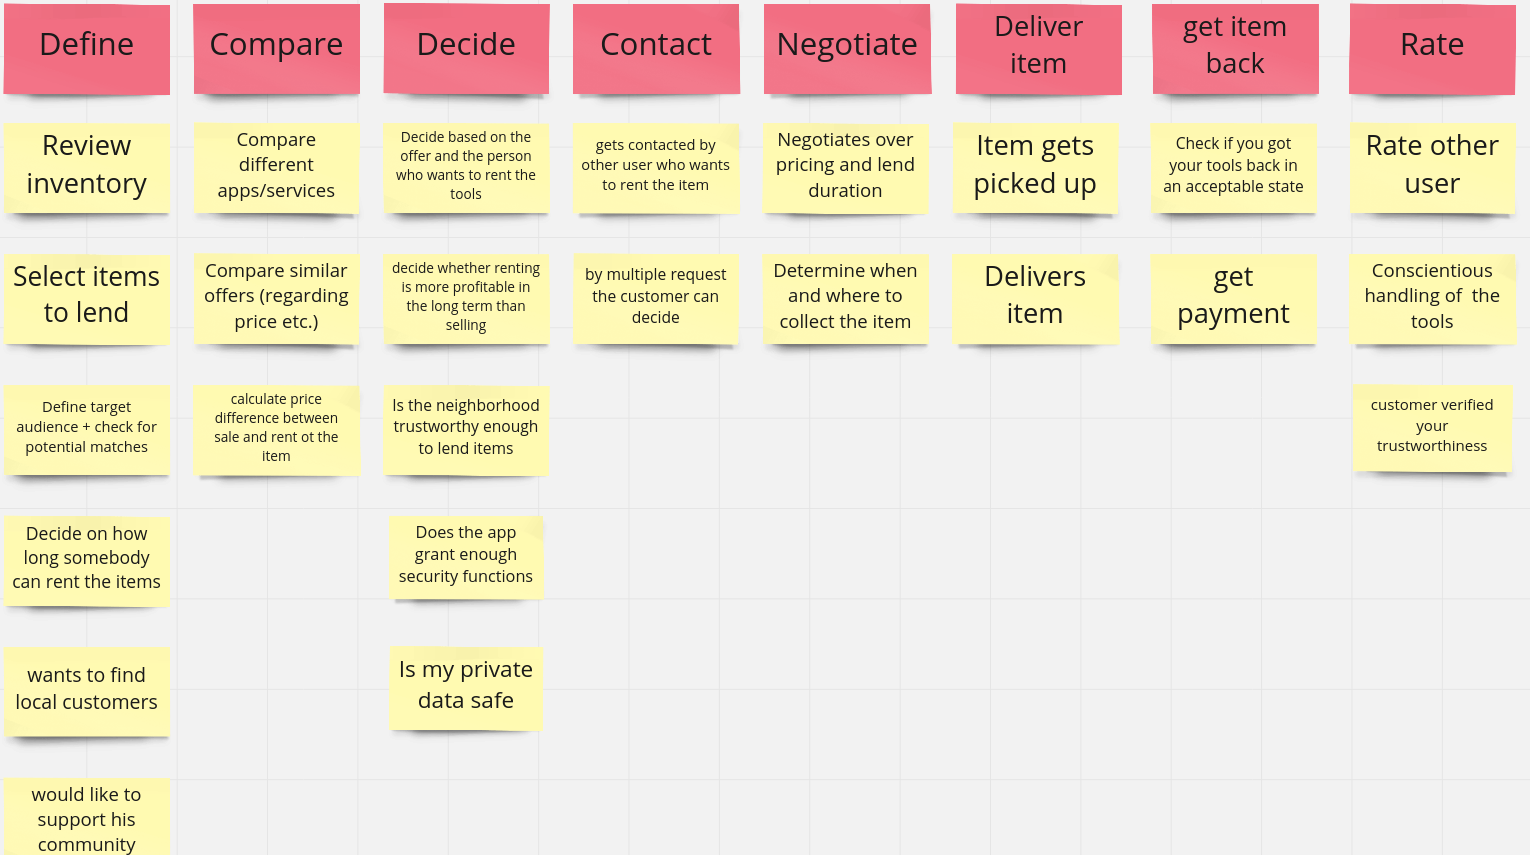
\includegraphics[width=\linewidth]{abb/2_context_of_use/user_journey_map_lending.png}
				\caption{User journey map for lending user}
				\label{fig:ujm_lending}
			\end{figure}
		
			\begin{figure}[H]
				\centering
				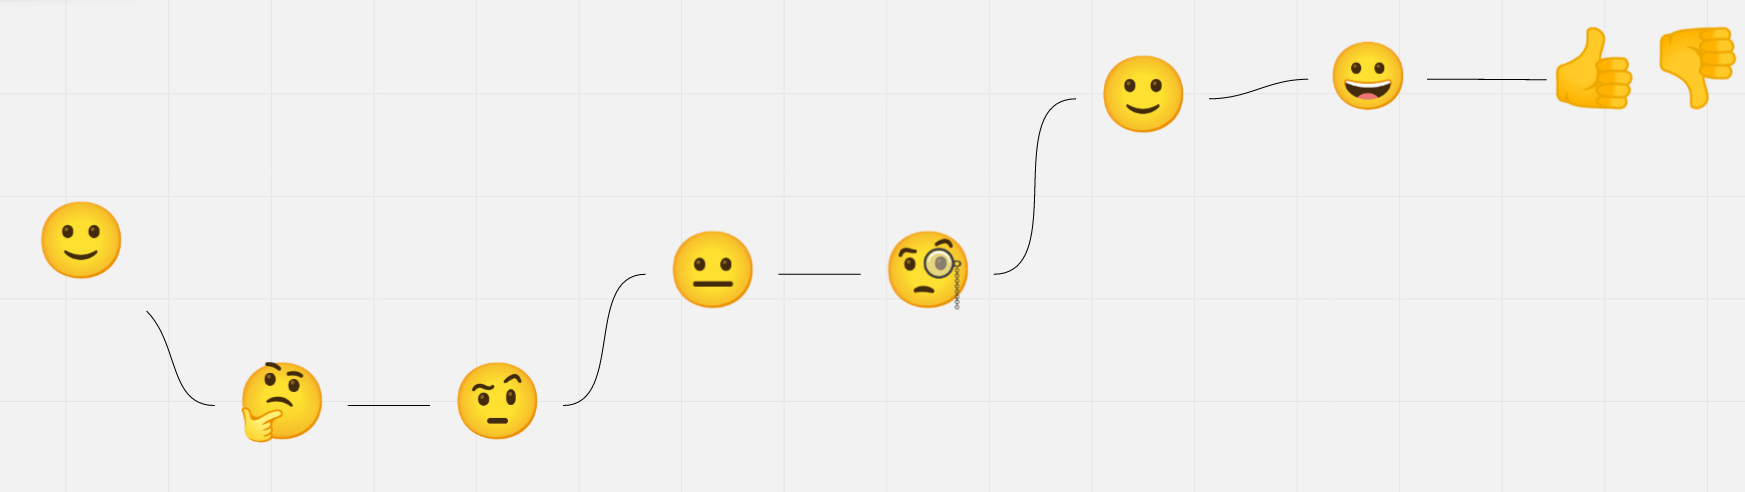
\includegraphics[width=\linewidth]{abb/2_context_of_use/feelings_lending.png}
				\caption{Feelings for renting user}
				\label{fig:ujm_lending_feelings}
			\end{figure}

\subsection{User Stories}

\definecolor{role}{HTML}{fac710}
\definecolor{goal}{HTML}{cee741}
\definecolor{benefit}{HTML}{2D9BF0}

User stories were developed to precisely identify the needs of the users in their roles. To illustrate this, the stories were listed in a mind map. Here, the map can be read from the inside out as follows:\\
\textbf {As a \colorbox{role}{<role>} I want \colorbox{goal}{<goal>} so that \colorbox{benefit}{<benefit>}}\\
The stories are sorted from top to bottom by importance.

\subsubsection{Stories for the renter}
\begin{figure}[H]
	\centering
	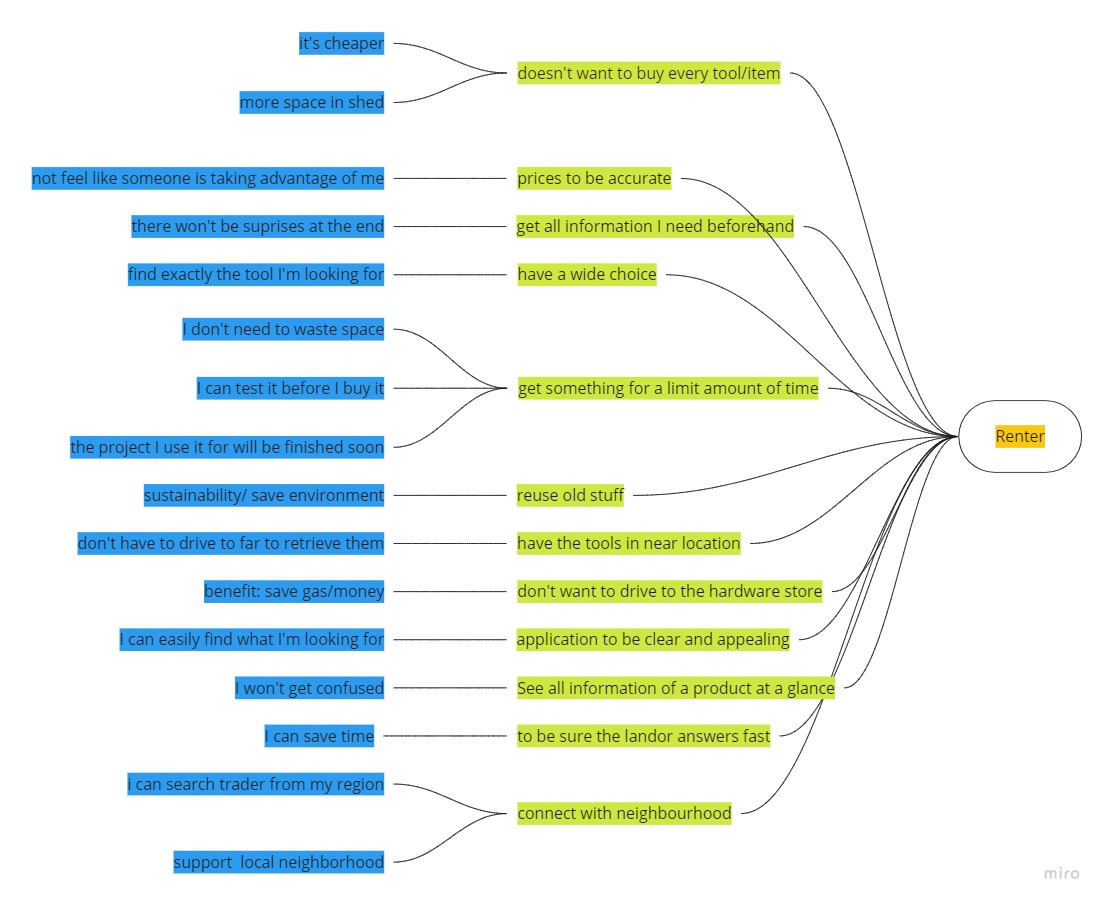
\includegraphics[width=\linewidth]{abb/2_context_of_use/story_renting.jpg}
	\caption{Renter Story}
	\label{fig:story_renter}
\end{figure}


\subsubsection{Stories for the lender}
\begin{figure}[H]
	\centering
	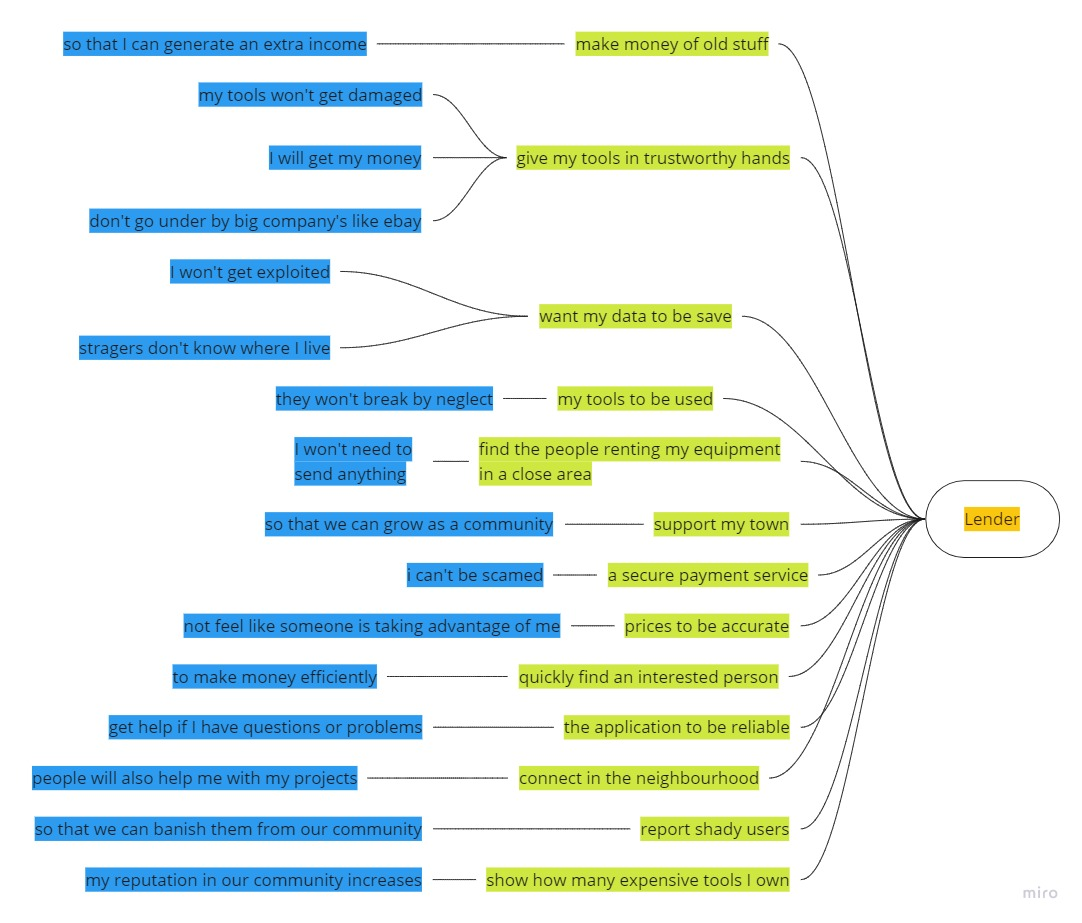
\includegraphics[width=\linewidth]{abb/2_context_of_use/story_lending.jpg}
	\caption{Lender Story}
	\label{fig:story_lender}
\end{figure}

